%!TEX root = ../thesis.tex
%*******************************************************************************
%*********************************** Introduction *****************************
%*******************************************************************************

\chapter{Introduction}\label{cha:introduction}

\graphicspath{{01_Introduction/Figs/}}

\section{Infectious diseases}

\subsection{The nature of infectious diseases}

Infectious diseases are caused by pathogens:\ microorganisms such as viruses, bacteria, or fungi which spread from one individual to another. Pathogens may transmit directly from person-to-person (in the case of respiratory and blood-borne pathogens), or indirectly (as for vector-borne pathogens)~\parencite{Leung2021-wd}. Once a pathogen enters the body it invades cells and multiplies, and this process of infection can lead to illnesses ranging in severity from mild to life-threatening~\parencite{Alberts2002-zu}. The classic model of infectious disease considers a combination of three areas:\ the infectivity and virulence of the pathogen, the susceptibility of the individual, and their vulnerability due to environmental factors~\parencite{van-Seventer2017-rt}.

Infectious diseases play a significant role in the global burden of disease, and, given their disproportionate impact on vulnerable populations and outbreak potential, are a key area for public health research~\parencite{GBD-2019-Diseases-and-Injuries-Collaborators2020-gy}. The vector-borne infectious disease malaria has had perhaps the greatest impact of any infectious disease in history, causing the deaths of an estimated 1 in 10 affected individuals during the 19th century~\parencite{Carter2002-cu}. Malaria continues to affect millions worldwide and, alongside Human Immunodeficiency Virus (HIV)\nomenclature[z]{HIV}{Human Immunodeficiency Virus}, \textit{Mycobaterium tuberculosis} (MTB)\nomenclature[z]{MTB}{\textit{Mycobaterium tuberculosis}}, and emerging infectious diseases such as severe acute respiratory syndrome coronavirus 2 (SARS-CoV-2)\nomenclature[z]{SARS-CoV-2}{Severe acute respiratory syndrome coronavirus 2}, is nowadays among the leading causes of mortality globally~\parencite{van-Seventer2017-rt}.

\subsection{Key concepts in epidemiology}

Epidemiology is the study and analysis of patterns of diseases and determinants of health in a population. In the context of infectious diseases, epidemiologists and statisticians employ several standard measures of disease burden to assess the impact of a disease, and to guide the appropriate public health response. These measures include~\parencite{Coggon1978-no}:

\begin{enumerate}
  \item the \textbf{incidence of infection}, defined as the rate of new infections occurring over a specific period time, e.g.\ new cases per 1,000 people per year;
  \item the \textbf{prevalence of infection}, defined as the proportion of the population that have the disease at a specific point in time, regardless of when they became infected;
  \item for diseases with adverse outcomes, the \textbf{mortality associated with infection}, defined as the incidence of death from the disease.
\end{enumerate}

A key measure of the spread of a disease, related to the incidence of infection, is the basic reproduction number, denoted $R_0$. The $R_0$ value measures the expected number of cases directly generated by one case in a population where all individuals are susceptible to infection~\parencite{Lipsitch2003-hb}. For instance, if $R_0 = 3$ for a particular disease then one infected individual will, on average, infect three others. When $R_0>1$ an infection will spread in a population, whereas when $R_0<1$ the infection will eventually die out.

Importantly, not every individual within a population will be equally susceptible to infection. Immunity to a pathogen might be acquired through vaccination or recovery from previous infection, both of which can provide a level of protection against future infections. Through widespread vaccination, immunity can be conferred to a large portion of a population, reducing susceptibility and thereby decreasing $R_0$~\parencite{Mongin2023-gj}.

\subsection{Historic and contemporary epidemics}

The terms epidemic, pandemic, and endemic are used to describe the geographical spread and prevalence of infectious diseases. Epidemic refers to an increase in the number of cases of a disease, above what is usually expected; a pandemic is an epidemic which has crossed country borders and affects a large proportion of people; and endemic is the constant or usual prevalence of a disease within a geographic area~\parencite{van-Seventer2017-rt}.

\subsubsection{The bubonic plague epidemic:\ 1346--1352}

The bubonic plague, also known as the `Black Death', is a notable example of a severe and highly infectious epidemic. Caused by the bacterium \textit{Yersinia pestis}, which is spread by fleas living on small mammals, the Black Death epidemic that spread through Europe between 1346 to 1352 had an estimated mortality rate of up to 60\%~\parencite{Benedictow2004-nc}.

\subsubsection{The HIV epidemic:\ 1981--today}

A more recent epidemic is that of Human Immunodeficiency Virus (HIV)\@. HIV is a retrovirus that targets the immune system, particularly CD4+ (Cluster of differentiation 4)\nomenclature[z]{CD4}{Cluster of differentiation 4} T cells, and is transmitted through contact with blood or other bodily fluids; most often via sexual contact, contact with blood and blood products, or vertically from mother to child~\parencite{Delpech2022-af}. Without effective treatment, HIV infection leads to a progressive decline in CD4+ T cells, resulting in a weakened immune system and increased susceptibility to opportunistic infections and cancers; a condition known as Acquired Immune Deficiency Syndrome\nomenclature[z]{AIDS}{Acquired Immune Deficiency Syndrome}~\parencite{Lipman2006-xd}.

The first cases of AIDS illness were reported among young men in Los Angeles in 1981~\parencite{The_Lancet2021-sq}, and the viral cause discovered in 1983~\parencite{Gallo1984-ci, Barre-Sinoussi1983-mt}. According to statistics from the~\cite{Joint_United_Nations_Programme_on_HIVAIDS_UNAIDS2023-sl}, since the start of the HIV epidemic, 85.6 million (95\% confidence interval (CI)\nomenclature[z]{CI}{Confidence interval} 64.8 to 113.0 million) people have acquired HIV worldwide, and 40.4 million (95\% CI 32.9 to 51.3 million) have died from AIDS-related illnesses. HIV remains an urgent issue in much of the world, with substantial disparity between regions --- adult HIV prevalence in sub-Saharan African countries with endemic HIV may exceed 15\%, whereas prevalence in many western European countries is below 0.1\%~\parencite{Joint_United_Nations_Programme_on_HIVAIDS_UNAIDS2023-ht}.

\subsubsection{The COVID-19 pandemic:\ 2020--2023}

The most widespread pandemic of modern times has been coronavirus disease 2019 (COVID-19)\nomenclature[z]{COVID-19}{Coronavirus disease 2019}. First detected in November 2019 in Wuhan, China, the SARS-CoV-2 virus which causes COVID-19 would subsequently spread to all areas of China, then around the world~\parencite{South_China_Morning_Post2020-dv}. SARS-CoV-2 was designated a Public Health Emergency of International Concern by the World Health Organisation (WHO)\nomenclature[z]{WHO}{World Health Organisation} in January 2020, and officially declared a pandemic in March 2020, a designation which would last for more than 3 years, with the impact of COVID-19 felt in every country around the globe~\parencite{World_Health_Organisation2020-uq, World_Health_Organisation2023-yr}.

Although unclear at the time, it is now known that SARS-CoV-2 is primarily transmitted through airborne virus particles, with symptoms usually appearing within 1--2 days of infection~\parencite{UK-Health-Security-Agency2022-vp}. Most people recover from SARS-CoV-2 infection, but it can be a fatal condition, especially for those with pre-existing comorbidities~\parencite{Docherty2021-es}.

As of March 2024, there have been 775 million confirmed cases of COVID-19 globally, and more than 7 million deaths attributed to the disease~\parencite{World_Health_Organization2020-lp}. The total number of infections is likely to be substantially higher, however, due to a combination of under-reporting of confirmed cases and insufficient testing capacity for symptomatic cases.

\section{Public health response to infectious diseases}

Whilst the characteristics, infection mechanisms, and scale of the HIV and SARS-CoV-2 epidemics are dissimilar, parallels can be drawn:\ both viruses arose from an unknown (probable zoonotic) source~\parencite{Contini2020-gk}, both have caused extreme prejudice towards marginalised communities~\parencite{Hibbert2018-hz, Bhanot2020-tp}, and government intervention and new public health measures have been required to mitigate the impact on healthcare services~\parencite{Brauner2021-np, Brown2018-nk}.

\subsection{Strategies for infectious disease prevention and control}\label{sec:prevention-strategies}

Given the immense global impact of both HIV and SARS-CoV-2, the importance of the public health response and efforts to effectively prevent, diagnose, and manage infectious diseases cannot be overstated. In May 2020,~\cite{Hargreaves2020-hr} proposed three `lessons learnt' from the HIV epidemic for the COVID-19 response:\ anticipating health inequalities; supporting behavioural changes; and multidisciplinary efforts to design and evaluate public health interventions. The public health interventions applied in both epidemics have so far included:\ testing, physical barriers, social distancing, and pharmaceutical interventions.

\subsubsection{Testing, physical barriers, and social distancing}

The United Kingdom (UK)\nomenclature[z]{UK}{United Kingdom} has a long history of HIV prevention and control. In 1986, the UK became one of the first countries to introduce a national needle exchange programme, designed to reduce HIV transmission among people who inject drugs~\parencite{Vlahov1998-qe}. `Don't Die of Ignorance', a national HIV prevention campaign, launched the following year in the UK (Figure~\ref{fig:aids-leaflet}) and has been credited with raising awareness of HIV and AIDS among the general public~\parencite{Fowler2014-cx}.

\begin{figure}[htbp!]
  \centering
  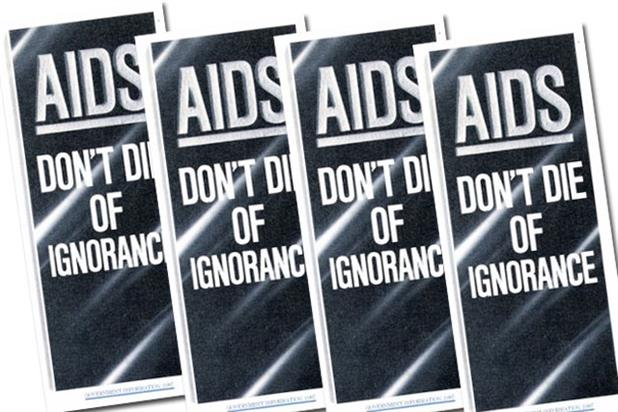
\includegraphics[width=0.5\textwidth]{aids-leaflet.jpg}
  \caption[AIDS:\ Don't die of ignorance leaflets sent to all British households in 1987]{AIDS:\ Don't die of ignorance leaflets that were sent to all British households in 1987\@. \textit{Source: www.campaignlive.co.uk}.}\label{fig:aids-leaflet}
\end{figure}

Testing is vital to the public health response to HIV, since early diagnosis provides the best opportunity for treatment initiation and prevention interventions to limit onward transmission~\parencite{Cohen2010-ol}. In recent years, public health guidelines have recommended that all patients in `high' (>2 per 1,000) and `very high' (>5 per 1,000) diagnosed prevalence areas be offered routine HIV testing when accessing healthcare services or registering with a general practitioner (GP)\nomenclature[z]{GP}{General practitioner}~\parencite{Health-Protection-Agency2011-ek, Gulland2011-fb, National_Institute_for_Health_and_Care_Excellence2016-js}.

Today, HIV prevention policies advocate for a combination of strategies, including regular community point of care testing, self-testing, and home-testing~\parencite{National_Institute_for_Health_and_Care_Excellence2016-js}, as well as condom usage~\parencite{Pebody2021-fb}, partner notification, and pharmaceutical interventions. Campaigns to normalise regular HIV testing, such as European Testing week, are run each year with promotion by UK-based third-sector organisations~\parencite{European_Testing_Week2023-ab}.

Testing has also formed the cornerstone of the response to the COVID-19 pandemic, with the number of weekly polymerase chain reaction (PCR)\nomenclature[z]{PCR}{Polymerase chain reaction} tests undertaken in England being scaled up to over a million per week during the initial months of the pandemic~\parencite{UK_Government2021-ip}. Individuals who tested positive were instructed to self-isolate for up to 10 days at home to reduce the risk of passing on the infection~\parencite{UK-Health-Security-Agency2022-lu}. Other interventions aimed at containing the spread of the virus included:\ social distancing guidance (Figure~\ref{fig:covid-distancing}); advice on the use of face masks and hand-washing; and local and national `lockdowns' which encompassed restrictions on movement and the closure of schools, workplaces, and hospitality venues~\parencite{Knock2021-ba}.

\begin{figure}[htbp!]
  \centering
  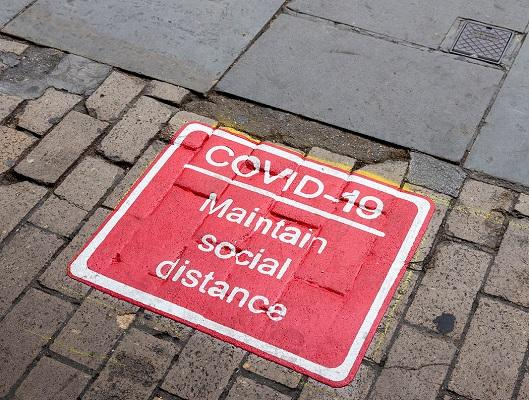
\includegraphics[width=0.5\textwidth]{covid-distancing.jpg}
  \caption[Social distancing notice on a pavement in Cambridge, UK]{Social distancing notice on a pavement in Cambridge, UK\@. \textit{Source: www.cambridgenetwork.co.uk}.}\label{fig:covid-distancing}
\end{figure}

\subsubsection{Treatment and vaccination programmes}

Once developed, pharmaceutical interventions including vaccination and treatment can be highly effective, if costly, tools to reduce the longer-term impact of infectious diseases~\parencite{Schrappe1998-py}. Monitoring their effectiveness in the real-world is, therefore, a major focus of public health research~\parencite{UK_Health_Security_Agency2021-gw}.

In the early years of the HIV epidemic, being diagnosed with HIV was considered a death sentence~\parencite{Rothenberg1987-hs,Pezzotti2003-kp,Collaborative_Group_on_AIDS_Incubation_and_HIV_Survival2000-wg}, and, while no cure currently exists, the introduction of effective antiretroviral therapy (ART)\nomenclature[z]{ART}{Antiretroviral therapy} in the mid-1990s, which suppresses the HIV virus in the body, has transformed HIV into a manageable, if chronic, condition~\parencite{Deeks2013-kl}. Provided they are diagnosed early in infection and adhere to treatment, the life expectancy of people diagnosed with HIV is now comparable to that of the general population~\parencite{Nakagawa2013-wa}. With treatment access becoming more widespread across HIV-endemic regions of sub-Saharan Africa, the number of AIDS-related deaths worldwide has plummeted; from an estimated 1.3 million (95\% CI 970,000 to 1.8 million) in 2010 to 630,000 (95\% CI 480,000 to 880,000) in 2022~\parencite{Joint_United_Nations_Programme_on_HIVAIDS_UNAIDS2023-sl}.

ART is also an effective way of preventing onwards transmission of HIV, with studies demonstrating that individuals with an undetectable viral load are unable to pass on HIV (known as undetectable = untransmittable, or U=U\nomenclature[z]{U=U}{Undetectable = untransmittable})~\parencite{World_Health_Organization2023-xi, Cohen2016-wy}. As part of combination prevention, pre-exposure prophylaxis (PrEP)\nomenclature[z]{PrEP}{Pre-exposure prophylaxis}, which can help to prevent HIV acquisition for a HIV-negative individual, has been targeted towards key HIV prevention groups in the UK and worldwide~\parencite{Brown2017-yu, Rivet-Amico2019-di}.

The development of pharmaceutical interventions for SARS-CoV-2 has been incredibly rapid, with an unprecedented international effort by private and public institutions~\parencite{Krammer2020-yo}. As a result, less than a year after the detection of SARS-CoV-2, two COVID-19 vaccine candidates were granted approval in the UK~\parencite{Sharma2020-jt, Medicines_and_Healthcare_products_Regulatory_Agency2020-jn}. Within a year of this approval, 40 million people in England had received two vaccine doses, and 30 million had also received a third dose~\parencite{UK_Government2021-ip}. This extensive vaccination campaign dramatically changed the outlook for COVID-19 in England, reducing the risk of infection, lessening symptoms, and reducing morbidity and mortality for those who became infected~\parencite{Lopez_Bernal2021-gt, Public_Health_England2021-xs, Hall2021-si}.

\subsection{The role of surveillance data}

In the context of public health, surveillance data play a pivotal role in monitoring and responding to infectious diseases. The UK Health Security Agency (UKHSA)\nomenclature[z]{UKHSA}{United Kingdom Health Security Agency} is responsible for infectious disease monitoring and surveillance in the UK as part of its mission to prepare for, prevent, and respond to health threats, with the goal of saving lives and protecting livelihoods~\parencite{UK_Health_Security_Agency2023-jp}.

Surveillance data can take various forms, including case and aggregate reporting. Case reporting involves the collection of detailed individual-level data about each case of a disease, such as demographic information, clinical symptoms, and outcomes. Aggregate reporting, meanwhile, involves the collection of summary data about groups of cases~\parencite{Murray2017-me}. In emerging public health threats, timely case-surveillance data enable rapid response by local public health teams, e.g.\ helping to pinpoint outbreaks of diseases such as measles, and isolating individuals who may be affected to prevent further spread~\parencite{Jajosky2004-wr}. Case-surveillance data can also provide a comprehensive picture for routine monitoring of infectious diseases, enabling record linkage over time, and follow-up of individuals through different care pathways~\parencite{Trostian2022-lx}.

National public health agencies such as UKHSA routinely publish surveillance data as national statistics. These provide a snapshot of the current state of infectious diseases within the country, trends in recent years, and are used to inform public health policies~\parencite{UK-Health-Security-Agency2020-wc}. At an international level, the World Health Organisation (WHO) plays a similar role in the monitoring of infectious disease, collecting data from countries and providing a global perspective on infectious diseases~\parencite{World_Health_Organization2020-lp}.

\section{Estimating the burden of infectious disease}

To understand how quickly a virus is spreading through a population, and the corresponding burden of disease, timely and robust estimates are required~\parencite{De-Angelis2015-uy}. The incidence of new cases, prevalence of undiagnosed infection, and extent of disease severity can all inform policy makers seeking to implement effective and appropriate public health measures.

\subsection{Incidence and prevalence}

Incidence of infection and the prevalence of an infectious disease in a population are generally unobserved, with observable information restricted to testing outcomes among subsets of a population. Testing processes may themselves be influenced by unobserved parameters, such as an individual's propensity to test, and the time from infection to symptom presentation (if symptoms present at all)~\parencite{Lewis2017-lt}.

To reconstruct the incidence and prevalence of infection from the available testing data, statistical and mathematical modelling techniques which adjust for sampling biases are employed. These techniques combine information from a range of sources to make valid statistical inference about unobserved incidence and prevalence~\parencite{Karon2008-pd, Hallett2008-et}.

\subsection{Severity}

Common metrics to understand the severity of infectious diseases and the factors associated with adverse outcomes are the infection fatality risk (IFR)\nomenclature[z]{IFR}{Infection fatality risk} and case fatality risk (CFR)\nomenclature[z]{CFR}{Case fatality risk}. The IFR is defined as the conditional probability of death given infection, whilst the CFR is defined as the conditional probability of death given a \textit{confirmed case} of infection~\parencite{Perez-Guzman2023-ih}. Since infections resulting in death are more likely to be recorded, and mild infections (particularly asymptomatic infections) less likely to be recorded, the CFR will almost always be higher than the IFR\@. Statistical modelling can be used to relate these measures of severity to underlying characteristics collected through case-surveillance data~\parencite{Wong2013-aq}.

\subsection{Effectiveness of interventions}

Monitoring outcomes among a target group after the introduction of a public health intervention allows for the real-world effectiveness of the intervention to be assessed, and changes over time to be detected. For example, effectiveness estimates might consider reductions in the transmission or acquisition of an infection among a treated group. Making these estimates requires reliable testing data, recognition of potential biases, and methodologies which can account for these biases~\parencite{Brauner2021-np}.

\subsection{Challenges in estimating infectious disease burden}

The majority of the data available for infectious disease monitoring relies on observational data, where a population is followed without actively intervening on an exposure~\parencite{Baker2023-me}. As a result, estimates of infectious disease burden are often considerably complicated by selection bias, which arises when the selected population observed is different from the general population of interest.

Common causes of selection bias include:\ testing policies (which may vary nationally and sub-nationally), individual health-seeking behaviour, test availability, clinician decision-making, and detection rates of different tests~\parencite{Hernan2004-ht}. Inaccuracies in the available case-surveillance data may also arise:\ at data input, due to incomplete/inaccurate reporting or misdiagnosis; and at data collection, due to insufficient surveillance infrastructure and data processing methods.

Unless the potential sources of bias are well-understood and accounted for they can affect the validity of estimates~\parencite{Westreich2012-kq}. For example, the IFR measure of severity requires complete knowledge of both the number of infections and number of deaths. Particularly in the early stages of a pandemic, when testing is either unavailable or sub-optimal, these quantities may be impossible to measure. The CFR is more straightforward to assess, since confirmed infections are more likely to be recorded, but this measure is highly sensitive to testing. This was particularly the case during the initial wave of the COVID-19 pandemic, when biases in case-surveillance led to wide variability in national estimates of the case-fatality rate, from 0.1\% to over 25\%~\parencite{World_Health_Organization2020-kc, UK-Health-Security-Agency2020-wc}.

Even when knowledge of these multi-faceted biases is available, statistical methodologies must be carefully chosen to properly control for the biases.

\subsection{The role of multi-state models}

Multi-state models are a type of statistical model which may be used to describe health-related processes over time, particularly those relating to disease epidemics~\parencite{van-den-Hout2016-xy, Vynnycky2010-md}. The benefit of multi-state models for these applications is their flexibility, which allows for a wide array of disease processes to be modelled~\parencite{Hougaard1999-rw}. In a multi-state model, an individual begins in a given state, spends a period of time in that state, before moving to the next state. Figure~\ref{fig:basic-msm} shows a three-state model where individuals move between states 1, 2, and 3 according to transitions $\left\{q_{r,s} : r,s \in (1,2,3)\right\}$.

\begin{figure}[htbp!]
  \centering
  \begin{tikzpicture}
    \node[state, align=center] (A) {State\\1};
    \node[state, align=center] (B) [right = 30mm of A] {State\\2};
    \node[state, align=center] (C) [below left = 15mm and 8mm of B] {State\\3};

    % Edges
    \path (A) edge[bend left=20] node {$q_{1,2}$} (B);
    \path (B) edge[bend left=20] node {$q_{2,1}$} (A);
    \path (B) edge[bend left=20] node {$q_{2,3}$} (C);
    \path (A) edge[bend right=20] node['] {$q_{1,3}$} (C);
  \end{tikzpicture}

  \caption[Example of a three-state model]{Example of a three-state model with transitions between states according to transitions $\left\{q_{r,s} : r,s \in (1,2,3)\right\}$.}\label{fig:basic-msm}
\end{figure}

Multi-state survival models can be used to model linear processes (e.g.\ disease progression), cyclic processes (e.g.\ infection and recovery), and may include absorbing states, such as death~\parencite{Andersen2002-uv}. As with any statistical model, a detailed understanding of the data-generating processes for the available data compared to the target population, and careful model specification is required to control for potential sources of bias~\parencite{Westreich2012-kq}. However, by incorporating information on intermediate events, these models can provide a more nuanced understanding of disease progression and the effect of interventions than classic survival analyses (see Section~\ref{sec:multi-state-models} for further details).

Specific recent applications of multi-state models to infectious disease epidemics have included HIV, pandemic influenza, and COVID-19~\parencite{Brizzi2019-yj, Birrell2021-ou, Corbella2018-ka, Presanis2021-pv, Jackson2022-lt}.

\section{Objectives and thesis structure}

\subsection{Research aims and questions}

The research objective for my PhD is to develop statistical modelling approaches which can be applied to public health data, thereby enhancing our collective understanding of ongoing disease epidemics and providing evidence for decision makers and the wider community.

Specifically, I aim to apply multi-state survival models to estimate key quantities of infectious disease burden and the effectiveness of public health interventions in three areas:
%
\begin{enumerate}
  \item the incidence of HIV among gay and bisexual men in England, and trends in HIV incidence and undiagnosed HIV prevalence over time;
  \item the severity of COVID-19 among individuals hospitalised with the disease at various stages of the pandemic;
  \item the effectiveness of SARS-CoV-2 vaccination against infection among a cohort of healthcare workers.
\end{enumerate}

\subsection{Thesis structure}

In this introductory chapter I have introduced key concepts in infectious disease research, with specific reference to two of the most urgent public health epidemics of our time:\ HIV and COVID-19. I have outlined challenges in estimating infectious disease burden, and the role that multi-state models can play. In the final section of this chapter I describe the data governance procedures I have followed when working with infectious disease data.

In Chapter~\ref{cha:methods} I detail the statistical methods involved in survival analysis and the multi-state survival models I have applied as part of my PhD research. The nature and biases of various epidemiological study designs are discussed, with an introduction to key concepts in causal inference from observational data.

In Chapter~\ref{cha:hivbackcalc} I describe the development of a disease-staged, multi-state HIV back-calculation model to provide a more nuanced interpretation of markers of HIV disease progression. I investigate the sensitivity of this model to interruptions in HIV testing and HIV transmission, as may have occurred during the COVID-19 lockdowns in England.

In Chapter~\ref{cha:hospitalseverity} I apply competing risks multi-state survival models to estimate trends in hospital pathways and lengths of stays in hospital for patients with COVID-19, before and after widespread vaccination. I estimate how the prognosis for hospitalised individuals has changed based on patient characteristics and hospital pressures, accounting for specific data biases.

In Chapter~\ref{cha:siren} I apply multi-state survival models for interval-censored data to estimate fourth dose SARS-CoV-2 vaccine effectiveness, and protection from prior infection, against symptomatic and asymptomatic infection in a cohort of healthcare workers. These models are set in a causal inference framework to estimate the causal effect of vaccination in this cohort.

Lastly, in Chapter~\ref{cha:conclusions}, I summarise the specific contributions of my research, explaining what was already known, what this thesis adds, and whether my research aims have been met. I also highlight future applications and areas for future methodological research.

\section{Data governance}

\subsection{Legal basis for data collection}

The data used in my PhD were collected and supplied by UKHSA via an honorary contract. Statutory instrument 2002 No.\ 1483 in The Health Service Regulations provides the legal basis for data handling by UKHSA\@. UKHSA is also obligated to comply with the rules and regulations set out in the General Data Protection Regulation (GDPR)\nomenclature[z]{GDPR}{General Data Protection Regulation}.

\subsection{Ethical approval}

The surveillance data used in Chapters~\ref{cha:hivbackcalc} and~\ref{cha:hospitalseverity} were collected by NHS England and the UK Health Security Agency, with permissions granted under Regulation 3 of The Health Service (Control of Patient Information) Regulations 2002, and without explicit patient permission under Section 251 of the National Health Service (NHS)\nomenclature[z]{NHS}{National Health Service} Act 2006. My research was classified as surveillance undertaken as part of UKHSA's legal responsibility to monitor infectious disease, and in response to an urgent public health emergency, and exempted from full ethical review by the UKHSA Research Support and Governance Office~\parencite{Kirwan2022-ka, Kirwan2022-za}.

For the SIREN study data used in Chapter~\ref{cha:siren}, ethical approval was granted by the Berkshire Research Ethics Committee on May 22, 2020. The study collected consent from all participants and is registered under ISRCTN clinical trial registry number:\ \href{https://doi.org/10.1186/ISRCTN11041050}{11041050}. The trial protocol was published by~\cite{Wallace2022-vs}.

\subsection{Data protection}

All of the data used in my PhD were stored and analysed under agreed data governance protocols, as set out below and in accordance with the Data Protection Act 2018~\parencite{Spencer2019-ga}.

Data sharing agreements, data permissions, and an honorary contract with UKHSA were required before receiving or processing any patient data. All patient-level data were stored securely on UKHSA network drives with restricted access on an encrypted UKHSA laptop. All data analyses were carried out on this laptop, or, where agreed under the data sharing agreements, fully anonymised summary datasets were encrypted and transferred for analysis on a secure University of Cambridge server with limited permissions. I undertook Caldicott training for data protection and completed UKHSA information governance training on an annual basis.

A data governance policy specific to HIV and STI surveillance systems is that no NHS numbers or patient names are collected. Instead, records are pseudoanyonymised, using a Soundex code (an algorithm for indexing names)~\parencite{Mortimer1995-ls} and first initial which allow for unique, non-identifying linkage of an individual's records between systems and over time~\parencite{Govuk2023-uj}. This policy did not impact upon my analyses of HIV data.

Over the course of my PhD, the UK national public health organisation transitioned from Public Health England\nomenclature[z]{PHE}{Public Health England} to UKHSA and I sought renewed permissions and an updated honorary contract to continue using the data.